\documentclass{standalone}
%<--------------------------------------------------------------------------->%
%%% TikZ %%%
\usepackage{tikz}
% \usetikzlibrary{calc}
% \usetikzlibrary{angles,quotes}
% \usetikzlibrary{intersections,topaths}
% \usetikzlibrary{decorations.markings}
%<--------------------------------------------------------------------------->%

\begin{document}

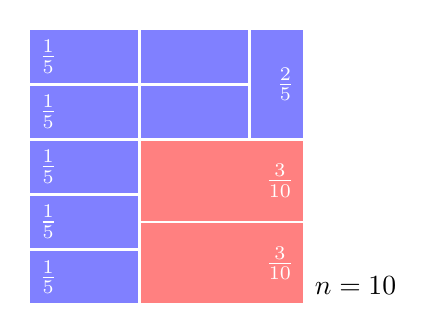
\begin{tikzpicture}[scale=3.5,thick,line cap=round]
	\tikzstyle{jiao}=[solid,circle,draw,fill=white,inner sep=.8pt];
	\tikzstyle{tile1}=[line width=0.1em,draw=white,fill=blue!50];
\tikzstyle{tile2}=[line width=0.1em,draw=white,fill=red!50];
\tikzstyle{tile3}=[line width=0.1em,draw=white,fill=blue!50!red!60];
\tikzstyle{tile4}=[line width=0.1em,draw=white,fill=blue!20!red!60];

	% \draw[tile1] (0,0)     rectangle (1,1);
	\draw[tile1] (0,0)     rectangle (2/5,1/5);
	\draw[tile1] (0,1/5)   rectangle (2/5,2/5);
	\draw[tile1] (0,2/5)   rectangle (2/5,3/5);
	\draw[tile1] (0,3/5)   rectangle (2/5,4/5);
	\draw[tile1] (0,4/5)   rectangle (2/5,1);
	\draw[tile1] (2/5,3/5) rectangle (4/5,4/5);
	\draw[tile1] (2/5,4/5) rectangle (4/5,1);
	\draw[tile1] (4/5,3/5) rectangle (1,1);
	\draw[tile2] (2/5,0)   rectangle (1,3/10);
	\draw[tile2] (2/5,3/10)   rectangle (1,6/10);
	\node[white,right] at (0,1/10) {$\frac{1}{5}$};
	\node[white,right] at (0,3/10) {$\frac{1}{5}$};
	\node[white,right] at (0,5/10) {$\frac{1}{5}$};
	\node[white,right] at (0,7/10) {$\frac{1}{5}$};
	\node[white,right] at (0,9/10) {$\frac{1}{5}$};
	\node[white,left] at (1,4/5) {$\frac{2}{5}$};
	\node[white,left] at (1,3/20) {$\frac{3}{10}$};
	\node[white,left] at (1,9/20) {$\frac{3}{10}$};
	\node[above right] at (1,0) {$n=10$};
\end{tikzpicture}

\end{document}
